\chapter{Results and Discussion}

The Engine and Transmission, and Braking modules both require that the Formula SAE 2010 vehicle be at least partly complete for testing. Since the build schedule for the vehicle is to have it complete for the beginning of May, 2010, much of the testing and tuning of these modules is incomplete.

The electronics for all four modules is completely implemented, tested and debugged. Most of the system software for all four modules has also been written.

\section{Transmission}

\subsection{Electro-pneumatic Simulation}


\subsection{System testing}

Since testing and tuning of the full electro-pneumatic system requires that the 2010 Formula SAE vehicle be complete, this phase of the project was not completed as intended, and is recommended for future work.


\section{Intake}


\section{Starter}


\section{Braking}


\subsection{Bias Adjustment}


\subsection{Calibration}


\section{Telemetry}

Getting the software implementation of the Telemetry module to work successufully was far more difficult than originally imagined. The individual components of the system software would run as expected on their own, but fail when coupled together. For example, the ECU data link and the DAC data link were at one point in the software development process relatively stable in operation by themselves, but enabling both would cause data loss, or one of the two links to drop. A large amount of time was invested in investigating the causes of these problems, and will be discussed in this section.

\subsubsection{Wireless Data Link}

We had originally planned to run the wireless link's data rate higher than \unit{115,200}{\bit\per\second}. The XBee documentation states that the modem is capable of running up to \unit{250,000}{\bit\per\second}, and the XBee modems allow for a continuous range of baud rates to be selected. Unfortunately it was determined when we started testing the Telemetry module software that the XBee could not in fact set it's baud rate to the highest possible with the MAX3100 was capable of: \unit{230,400}{\bit\per\second}.

The MAX3100 was therefore configured to operate at \unit{115,200}{\bit\per\second}, and the XBee modem's interface rate was matched. A simple throughput stress test was performed that continuously wrote data in 16 byte chunks into the MAX3100's driver's software transmit buffer. A fixed-length 32 byte software buffer was never overrun with this test, and an actual data throughput of $\unit{8.251}{\kilo\byte\per\second}$ was observed with a logic analyser on the TX pin of the MAX3100.

\subsection{Data Interfaces}

\subsubsection{ECU }

\subsubsection{DAC }



\subsection{Interrupt Starvation on the Telemetry Module}

Issues caused by the large degree of asynchronous behaviour in the system, and the large number of common resources used. Multiple producer/consumer layers. Solved by ensuring that atomic sections were placed around critical code.

Although initial average data throughput rates for both the DAC and the ECU were measured as part of the research done at the beginning of the project, non-trivial buffering issues did arise in the implementation of the telemetry module software. After several weeks of work spent debugging throughput problems with the module software, and with the aide of a protocol analyser, the root of the problem was tracked down. The AT90CAN microcontroller's interrupt vectors are fixed at the factory, therefore the priority of interrupts on the microcontroller is fixed. Unfortunately this lead to a resource starvation issue. The MAX3100 UART uses an external interrupt line, which has priority over the internal UART interrupts. When there is data in the MAX3100's transmit buffer, it will starve the internal UART interrupt to a certain extent. This was investigated by saturating the MAX3100 output buffer with a constant stream of data, and then inputting some bytes to the internal UART. Single input bytes were read properly, but any long stream of incoming bytes (more than 4 in a row) would cause hardware input buffer overruns in the built-in UART, and incoming data would be lost.

\begin{figure}[ht]
  \centering
  \label{fig:ecu_data}
  \begin{tikztimingtable} %[timing/nice tabs]
    $ECU_{Rx}$ & Z 10D{Polling sequence (7 bytes)} 14F Z \\
    $ECU_{Tx}$ & 12Z 6D{Reply sequence} ;[dotted] 2D{...}; 5D{(539 bytes)} Z\\
    \extracode
      %\tableheader{Signal}{Timing}
      \tablerules
  \end{tikztimingtable}
  \caption{ECU Serial Data Example}
\end{figure}

Based on this knowledge, we were able to classify conditions where the software would be unable to accurately process the incoming data. Unfortunately the method that the ECU transmits it's data falls within this characterization. When the ECU is communicating with the DTASWin software, the software will send a handful of bytes (around 7) to the ECU, and the ECU will reply with one large packet of approximately 540 bytes. If the MAX3100 is transmitting a large amount of data when this large packet comes in, bytes will be lost from the interrupt starvation issue.

Having determined the problem, several options lay before us to resolve the issue:
\begin{itemize}
  \item By lumping the ISR handlers for both the internal UART and the MAX3100 together, it would be possible to conditionally alter the priority of the processing to allow the incoming data to take precedence. This would however override the natural encapsulation that the two drivers had, and would require writing specialized drivers for use only on the telemetry module.
  \item Throttling the transmission of data to the MAX3100 by sequenced enabling and disabling of the interrupt could also reduce the starvation issue, but getting the sequencing and timing right would be difficult and more than likely result in further problems.
\end{itemize}


\section{Driver Interface}


\subsection{Driver Controls}


\subsection{Vehicle Dynamic Adjustment}


\subsection{Diagnostic Information}


\subsection{LCD Interface}

The memory-mapped LCD module interface, as described in \ref{sec:lcd_module_data_interface}, proved to be very useful in implementing the user interface software. By using GDB connected to the running Driver Interface module, it was possible to read and write data directly to the LCD by issuing GDB memory access commands. Several GDB macro scripts were set up

\subsubsection{Bench Experiments}

To verify the LCD data interface circuitry before the final Driver Interface module hardware had been completed, a bench test of the LCD module with an ARM7 development board was conducted. The bus interface as designed in Sec.\ \ref{sec:lcd_module_data_interface} was implemented on a breadboard: a latch and level shifter were used as in the Driver Interface module circuit design, and an FPC cable adapter was constructed with the aide of the tech shop to allow connecting the LCD module to the breadboard. The GPIO pins on the ARM7 development board (shown in red in Fig.\ \ref{fig:can_bench_test}) were used to bit-bang the data interface to the LCD. This test setup was used to write the initial LCD module code used in the final Driver Interface module implementation.

\begin{figure}[h!]
\centering
\subfigure[LCD Bench test]{
  \label{fig:lcd_bench_test}
  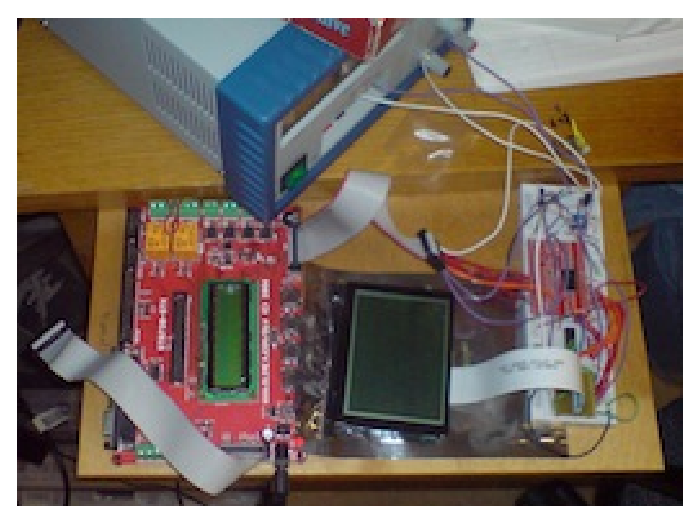
\includegraphics[width=2.5in,keepaspectratio]{results/figures/lcd_bench_test.eps}
}
\subfigure[CAN Bench test]{
  \label{fig:can_bench_test}
  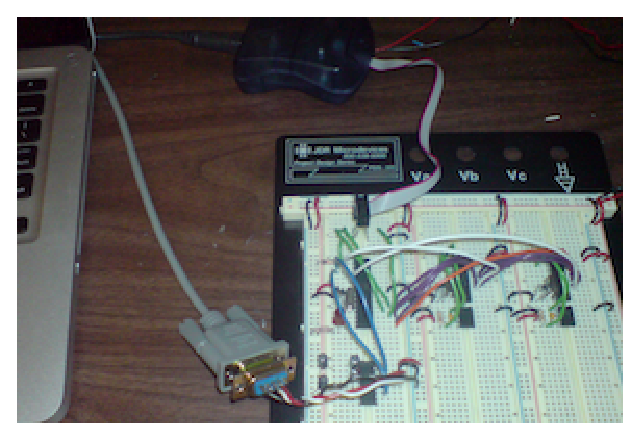
\includegraphics[width=2.5in,keepaspectratio]{results/figures/can_bench_test.eps}
}
\caption{Bench experiments conducted during the implementation phase.}
\label{fig:bench_experiments}
\end{figure}

Once all the hardware bugs with the Driver Interface module had been corrected, it was possible to continue writing the LCD interfacing software that had been started during the initial LCD testing. The external memory interface circuitry described in Sec.\ \label{sec:lcd_module_data_interface} worked without issue. Figure \ref{fig:driver_interface_lcd} shows the LCD displaying a sample bitmap from the manufacturer.

\begin{figure}[h]
 \centering
 \includegraphics[width=6in,keepaspectratio]{results/figures/driver_interface_lcd.eps}
 \caption{Testing the LCD on the Driver Interface module.}
 \label{fig:driver_interface_lcd}
\end{figure}

\section{Implementation Issues Encountered}


\subsection{Hardware Implementation Issues}


\subsubsection{CAN Transciever Schematic Error}


\subsubsection{Driver Interface LCD Reset Line}


\subsubsection{Telemetry RS-232 Transciever Schematic Error}





\subsection{CAN Driver Problems}